\documentclass{beamer}

\usepackage[utf8]{inputenc} % Language and font encoding
\usepackage[icelandic]{babel}
\usepackage[T1]{fontenc}


\usepackage{tikz}
\usepackage[listings,theorems]{tcolorbox}
\usepackage{booktabs}
\usepackage{minted} %Minted and configuration
\usemintedstyle{default}

\renewcommand{\theFancyVerbLine}{\sffamily \arabic{FancyVerbLine}}
%%%%%%%%%%%
% More math
%%%%%%%%%%%
\newcommand{\Mod}[1]{\ \text{mod}\ #1}

%%%%%%%%%%%%%%%%%%%%%%
% Beamer configuration
%%%%%%%%%%%%%%%%%%%%%%
\setbeamertemplate{navigation symbols}{}
\usecolortheme{dove}
\setbeamercolor{frametitle}{fg=white}

\usebackgroundtemplate%
{%
\vbox to \paperheight{

\includegraphics[width=\paperwidth]{Pics/hi-slide-head-2016}

\vfill
\hspace{0.5cm}
\includegraphics[width=0.3\paperwidth]{Pics/hi-von-logo}
\vspace{0.4cm}
    }%
}

\AtBeginSection[]
{
  \begin{frame}<beamer>
    \frametitle{Yfirlit}
    \tableofcontents[currentsection]
  \end{frame}
}

\setbeamerfont{frametitle}{size=\normalsize}
\addtobeamertemplate{frametitle}{}{\vspace*{0.5cm}}

%%%%%%%%%%%%%%%%%%%%%%%%%
% tcolorbox configuration
%%%%%%%%%%%%%%%%%%%%%%%%%

% Setup from: http://tex.stackexchange.com/a/43329/21638
\tcbset{%
    noparskip,
    colback=gray!10, %background color of the box
    colframe=gray!40, %color of frame and title background
    coltext=black, %color of body text
    coltitle=black, %color of title text 
    fonttitle=\bfseries,
    alerted/.style={coltitle=red, colframe=gray!40},
    example/.style={coltitle=black, colframe=green!20, colback=green!5},
}


%%%%%%%%%%%%%%%%%%%%%%%
% Further configuration
%%%%%%%%%%%%%%%%%%%%%%%
\hypersetup{colorlinks=true,pdfauthor={Eirikur Ernir Thorsteinsson},linkcolor=blue,urlcolor=blue}
\graphicspath{{./Pics/}}

\author{Eiríkur Ernir Þorsteinsson}
\institute{Háskóli Íslands}
\date{Haust 2016}

\title{Stærðfræðimynstur í tölvunarfræði}
\subtitle{Vika 2, fyrri fyrirlestur}

\begin{document}

\begin{frame}
\titlepage
\end{frame}

\section{Inngangur}

\begin{frame}{Í síðasta tíma}
\begin{itemize}
 \item Mengi!
 \begin{itemize}
  \item Stök í mengjum
  \item Hlutmengi
  \item Veldismengi og mengjamargfeldi
  \item Sniðmengi og sammengi
 \end{itemize}
\end{itemize}
\end{frame}

\section{Föll}

\begin{frame}{Föll}
\begin{itemize}
 \item Fall er hugtak sem er mörgum kunnuglegt úr stærðfræðigreiningu
 \begin{itemize}
  \item $f(x) = x^2$ er fall
  \item $\sin(x)$ er fall
 \end{itemize}
 \item Oftast hefur verið um að ræða föll sem taka inn eina rauntölu og skila annarri rauntölu
 \begin{itemize}
  \item Við notum opnari skilgreiningu
 \end{itemize}
\end{itemize}
\end{frame}

\begin{frame}{Skilgreining á falli}
\begin{tcolorbox}[title=Fall]
Látum $A$ og $B$ vera mengi sem eru ekki tóm. Fall (e. \emph{function}) $f$ frá $A$ til $B$ er ákvörðun á nákvæmlega einu staki í $B$ fyrir sérhvert stak í $A$.

Við skrifum $f(a) = b$ þegar $b$ er stakið sem fallið $f$ ákvarðar fyrir stakið $a$.

Við skrifum $f: A \to B$ þegar $f$ er fall frá $A$ til $B$.
\end{tcolorbox}

Föll eru líka kölluð varpanir (e. \emph{mapping} eða \emph{transformation}). Fall $f: A \to B$ varpar stökum úr mengi $A$ yfir í mengi $B$.
\end{frame}

\begin{frame}{Dæmi um föll}
\begin{itemize}
 \item Föll sem skilgreind eru með formúlu, föll með þekkt nöfn
 \begin{itemize}
  \item $f(x) = x^2$ er $\mathbf{R} \to \mathbf{R}$
  \item $\sin(x)$ er líka $\mathbf{R} \to \mathbf{R}$
 \end{itemize}
 \item Ákvörðun einkunna í þessu námskeiði má tákna með falli
 \item Ákvörðun nafna út frá kennitölum má tákna með falli \pause
 \begin{itemize}
  \item Ákvörðun kennitala út frá nöfnum er ekki fall!
 \end{itemize}
\end{itemize}
\end{frame}

\begin{frame}{Formengi og myndmengi}
\begin{tcolorbox}[title=Formengi og myndmengi]
Sé $f$ fall frá $A$ til $B$ kallast $A$ formengi (e. \emph{domain}) fallsins og $B$ myndmengi (e. \emph{codomain}) þess. Sé $f(a) = b$ er sagt að $b$ sé mynd (e. \emph{image}) $a$ og að $a$ sé formynd (e. \emph{preimage}) $a$.
\end{tcolorbox}
Sum föll eru hlutskilgreind (e. \emph{partial functions}), þ.e.a.s. að þau eru ekki skilgreind fyrir öll stök í formengi sínu. Dæmi: $f(x) = 1/x$.
\end{frame}

\begin{frame}[fragile]{Föll í forritun}
\begin{itemize}
 \item Föll eru gríðarlega mikið notuð í forritun, í ýmsum myndum
 \begin{itemize}
  \item Dæmigert fall í forritun:
  \begin{itemize}
   \item Tekur inn breytur
   \item Framkvæmir reikniaðgerðir
   \item Skilar niðurstöðu í samræmi við inntakið 
  \end{itemize}
 \end{itemize}
 \item Í mörgum forritunarmálum eru formengi og myndmengi tilgreind þegar fall er skilgreint
\end{itemize}
\begin{minted}[frame=lines]{java}
// Fall frá mengi strengja til mengi heiltalna
public static int f (String s) {
  ...
}
\end{minted}

\end{frame}

\begin{frame}{Eintæk föll}
\begin{tcolorbox}[title=Eintækt fall]
Fall er eintækt (e. \emph{injective}) ef það varpar engum tveimur stökum í formengi sínu í sama stak myndmengisins, þ.e.a.s. ef \[\forall a \forall b (f(a) = f(b) \to a = b)\] og þar með \[\forall a \forall b (f(a) \neq f(b) \to a \neq b)\].
\end{tcolorbox}
\end{frame}

\begin{frame}{Átæk föll}
\begin{tcolorbox}[title=Átækt fall]
Fall $f$ er átækt (e. \emph{surjective}) ef það ``þekur'' myndmengi sitt, þ.e.a.s. að fyrir hvert stak $b$ í myndmenginu er til stak í formenginu $a$ svo að $f(a) = b$, \[\forall b \exists a (f(a) = b)\].
\end{tcolorbox}
\end{frame}

\begin{frame}{Eintækni og átækni}
\begin{center}
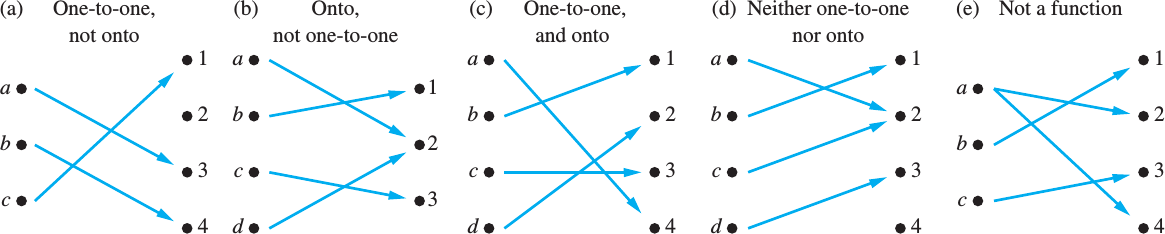
\includegraphics[width=\textwidth]{function-types}
\end{center}
Fall sem er bæði eintækt og átækt er kallað gagntækt.
\end{frame}

\begin{frame}{Andhverfanleg föll}
\begin{tcolorbox}[title=Andhverfanlegt fall]
Látum $f$ vera gagntækt fall frá $A$ til $B$. Þá er andhverfa fallsins $f$ fallið sem varpar $b \in B$ í stakið $a \in A$ sem um gildir að $f(a) = b$.

Andhverfa fallsins $f$ er táknuð með $f^{-1}$. Um $f^{-1}$ gildir:

\[
 f(a) = b \leftrightarrow f^{-1}(b) = a
\]

\end{tcolorbox}
\end{frame}



\section{Rakningavensl}

\section{Reiknanleiki}

\section{Fylki}

\begin{frame}{Næst}
Föll (kafli 2.3), rakningavensl (kafli 2.4), reiknanleiki (kafli 2.5), fylki (kafli 2.6)
\end{frame}


\end{document}
